% textidote: ignore begin
\section{Development process}\label{sec:development-process}
% textidote: ignore end

This section describes the different elements of the development process.
Other development processes and protocols exist in the team; however, only the most important ones are mentioned in the
following sections.

% textidote: ignore begin

\subsection{Development environment}\label{subsec:development-environment}
% textidote: ignore end

The project requires a number of different services to be running at the same time, which can be challenging to manage.
% textidote: ignore begin % Due to node.js being identified as an url
That is the Node.js backend, Stockfish and Firebase Emulator.
% textidote: ignore end
To manage them, the team uses Docker~\cite{docker} to simultaneously run all the services.
Docker is a platform that allows developers to isolate their applications in containers, which are lightweight and can
run on any machine on any operating system.
This makes it painless to develop multiservice projects, as there are no compatibility issues between the different
devices and services.
To handle multiple containers, the team uses Docker Compose, which is a tool for defining and running multi-container
Docker applications.
This makes it possible to run all the services locally when developing, simulating how they will behave in a production
environment.

% textidote: ignore begin

\subsection{CI/CD}\label{subsec:ci/cd}
% textidote: ignore end

The team uses GitHub~\cite{github} for version control and continued integration and development (CI/CD) for both the
report writing process and the development of the software.
GitHub provides many features, such as pull requests, issues, actions, and projects, which makes it easy to collaborate
and work on the project and the report.

The team uses branches, where the unwritten rules is that only the creator of the branch makes changes to the code in
the branch to avoid accidental overwriting of code.
Having branches makes it simple to track what team members are working on and how far in development they are.

\subsubsection{Task management}

The team makes use of GitHub projects to plan out different tasks and issues to track bugs and features.
A snapshot of some categories with some issues can be seen in Figure~\ref{fig:github-project}.
In the figure, it is clear that issues move from category to category as the team progresses with them.

The custom protocol is for a team member to assign one self to an issue and thereafter complete the task associated with
the issue.
This way, other team members can comment inside the issue if they have comments about what the issue entails.
Another reason for this method is that it is clear to all members what problems are being solved in a given pull request
as the relevant issue is linked, thereby improving efficiency and clarity.
This method of creating issue and assigning one self to them makes for a lot of freedom in development.

This freedom, however, comes with the responsibility for team members to adequately assign themselves to enough issues
to cover their respective workload commitments.
Having the list of issues dynamically update, as team members resolve them, makes for a clean and
comprehensible overview of how much work needs to be done, how much is in progress, and how much has been done.

% textidote: ignore begin
\begin{figure}[htb]
    \centering
    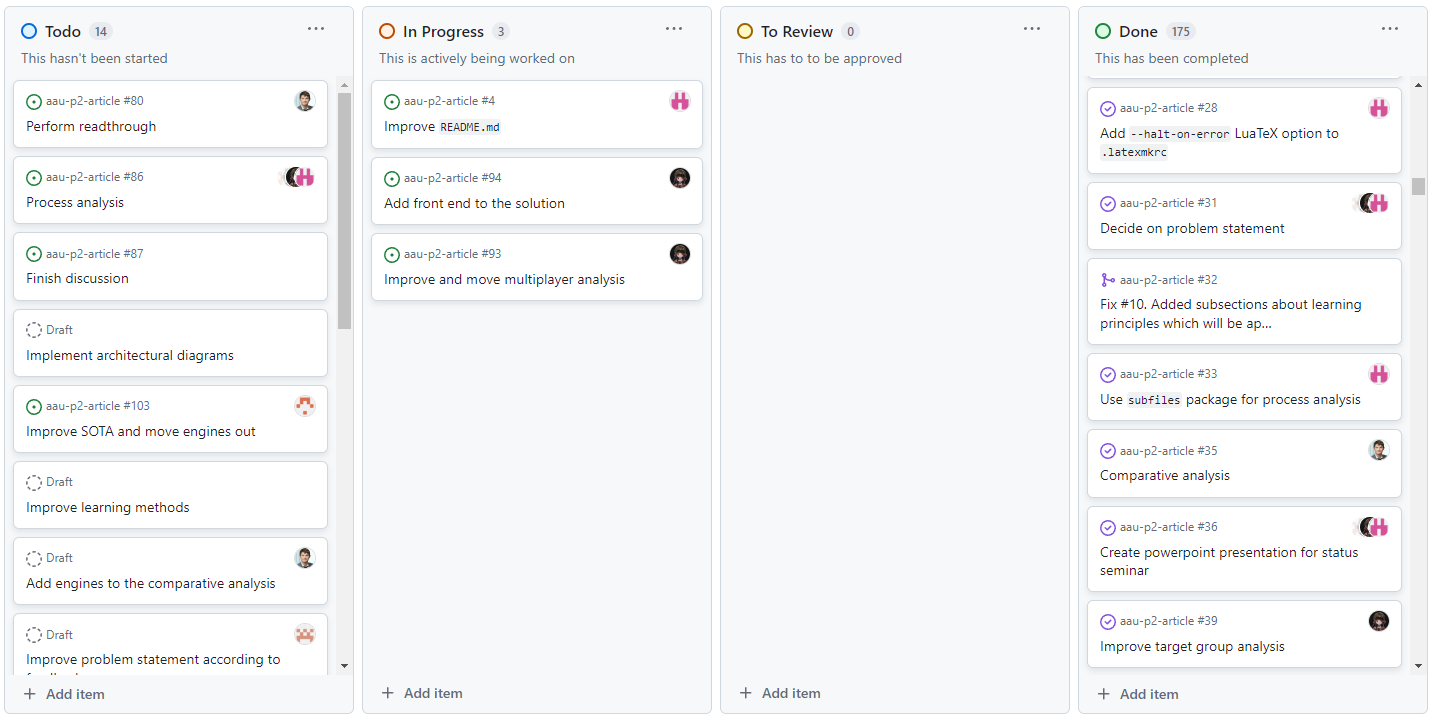
\includegraphics[width=1\textwidth]{github-projects}
    \caption{GitHub Project overview.}\label{fig:github-project}
\end{figure}
% textidote: ignore end

% textidote: ignore begin

\subsubsection{Automation}
% textidote: ignore end

GitHub Actions are used to run custom checks among others automatically.
Having the actions run on all lines of code makes for the security that other team members code is living up to the
standards desired and agreed on by the team.
Different actions are relevant for the four different repositories that make up the entire project codebase.
Reference to the repositories is made to Appendix~\ref{ch:source-code-repositories}.
The two repositories with the most changes throughout the development process are those for the report and the
front-end.
The focus is therefore on the actions for these, even though the other repositories also have GitHub Actions
attached to them.
In Table~\ref{tab:actions-overview} it can be seen that the team mainly uses five different actions.
In the table is also provided the main purpose of the action and a small description of them.

% textidote: ignore begin
\begin{table}[h]
    \centering
    \resizebox{\columnwidth}{!}{%
        \begin{tabular}{clllll}
            \toprule
            \rowcolor[HTML]{9B9B9B}
            \textbf{Actions} & \multicolumn{2}{c}{\cellcolor[HTML]{9B9B9B}\textbf{Attributes}} \\ \midrule
            \rowcolor[HTML]{EFEFEF}
            \cellcolor[HTML]{C0C0C0}{\color[HTML]{000000} \textit{\textbf{Report}}}    &
            \multicolumn{1}{c}{\cellcolor[HTML]{EFEFEF}\textbf{Purpose}}  &
            \multicolumn{1}{c}{\cellcolor[HTML]{EFEFEF}\textbf{Description}}
            \\ \midrule
            \cellcolor[HTML]{EFEFEF}\textbf{xu-cheng's latex-action}                   & \begin{tabular}[c]{l}
                                                                                             Compiles the latex document
            \end{tabular} & \multicolumn{1}{l}{\begin{tabular}[c]{l}
                                                   This action is made by a private person and runs \\
                                                   a docker container with TexLive installed
            \end{tabular}}                                 \\ \midrule
            \cellcolor[HTML]{EFEFEF}\textbf{TeXtidote}                                   & \begin{tabular}[c]{l}
                                                                                               Lints the latex document
            \end{tabular} & \multicolumn{1}{l}{\begin{tabular}[c]{l}
                                                   This action utilizes the TeXtidote binary to lint \\
                                                   the report for any spelling mistakes
            \end{tabular}} \\ \midrule
            \cellcolor[HTML]{EFEFEF}\textbf{Chk TeX}                                    & \begin{tabular}[c]{l}
                                                                                              Formats the latex document
            \end{tabular} & \multicolumn{1}{l}{\begin{tabular}[c]{l}
                                                   This action makes use of Chk TeX, which cheks for \\
                                                   common mistakes in latex\. We mostly use it to \\
                                                   format tables and images correctly
            \end{tabular}}                                  \\ \midrule
            \rowcolor[HTML]{EFEFEF}
            \cellcolor[HTML]{C0C0C0}{\color[HTML]{333333} \textit{\textbf{Front-end}}}
            & \multicolumn{1}{c}{\cellcolor[HTML]{EFEFEF}\textbf{Purpose}}        &
            \multicolumn{1}{c}{\cellcolor[HTML]{EFEFEF}\textbf{Description}}     \\ \midrule
            \cellcolor[HTML]{EFEFEF}\textbf{ESLint}                                  & \begin{tabular}[c]{l}
                                                                                           Lints the software
            \end{tabular}        & \multicolumn{1}{l}{\begin{tabular}[c]{l}
                                                          ESLint is used mostly for the best practise \\
                                                          comments it provides, such that the group follows \\
                                                          the same guidelines when coding
            \end{tabular}}                                  \\ \midrule
            \cellcolor[HTML]{EFEFEF}\textbf{Prettier}                                  & \begin{tabular}[c]{l}
                                                                                             Formats the software
            \end{tabular}        & \multicolumn{1}{l}{\begin{tabular}[c]{l}
                                                          Prettier makes sure that the code is indented \\
                                                          correctly among other formatting settings
            \end{tabular}}                                  \\ \bottomrule
        \end{tabular}%
    }
    \caption{Overview of the most used actions for the report and the software.}\label{tab:actions-overview}
\end{table}
% textidote: ignore end

These actions make for more efficient, more understandable and more reliable code, why they are used.

% textidote: ignore begin

\subsubsection{Quality control}
% textidote: ignore end

Another important process mechanism the team uses is the pull request feature of GitHub.
In the pull request is where changes to be merged into the main branch are displayed as well as where the GitHub Actions
runs are documented.
The custom protocol is for at least two team members to accept the changes made before the commits in the pull request
can be merged into the main branch.
This safety feature makes it such that at least three of the five team members agree with the changes made.
By having this barrier, it also makes sure that individual small changes can also be agreed on, and that they don't get
lost or go unseen by the rest of the team.

One of the advantages to using this method over software like Overleaf is that GitHub provides a log of all changes made
as well as ´blame'.
This makes it possible to see who made the changes at all times in local IDEs.
Being able to quickly identify the author of a line makes communication in the team more efficient.
One of the disadvantages is that development typically takes longer, as every change needs to be reviewed by the team
before being able to be merged.
This time delay can be a problem when approaching deadlines, however, in the big picture, it is not that big of an
issue.
